\documentclass[a4paper,english]{lipics-v2019}
\usepackage{wrapfig,microtype,amssymb,amsmath,stmaryrd,mathpartir,array,graphicx,tabularx,xspace}
\usepackage[table]{xcolor}
\newcommand{\xt}[1]{\texttt{#1}}
%\newcommand{\tupleo}[1]{\xt{Tuple1\{}#1\xt{\}}}
\newcommand{\tuplet}[2]{\xt{Tuple\{}#1,#2\xt{\}}}
\newcommand{\union}[2]{\xt{Union\{}#1,#2\xt{\}}}
\newcommand{\denotes}[1]{\llbracket #1 \rrbracket}

\renewcommand{\L}{{\tt L}\xspace}
\newcommand{\Ls}{{\tt L}s\xspace}
\newcommand{\R}{{\tt R}\xspace}
\newcommand{\Rs}{{\tt R}s\xspace}
\newcommand{\uL}{{\underline{\tt L}}\xspace}
\renewcommand{\c}[1]{\ensuremath{\text{\lstinline{#1}}}\xspace}

%FZ
\newcommand{\sub}{<:}
\newcommand{\tuple}[1]{\xt{Tuple\{}#1\xt{\}}}
\newcommand{\arrayt}[1]{\xt{Array\{}#1\xt{\}}}
\newcommand{\FZ}[1]{\textbf{FZ says: #1}}
%end FZ

\newcommand{\goodcell}{\cellcolor{green!25}}
\newcommand{\badcell}{\cellcolor{red!25}}
\bibliographystyle{plainurl}% the recommnded bibstyle
\title{Julia's efficient algorithm for subtyping unions and covariant tuples}
\titlerunning{Subtyping union types and covariant tuples}

\author{Benjamin Chung}{Northeastern University}{}{}{}%mandato
\author{Francesco Zappa Nardelli}{Inria}{}{}{} \author{Jan
  Vitek}{Northeastern University \& Czech Technical University in
 Prague}{}{}{}
\authorrunning{B. Chung, F. Zappa Nardelli, J. Vitek}
\Copyright{Benjamin Chung, Francesco Zappa Nardelli, Jan Vitek}%mandatory, plea
\ccsdesc[500]{Theory of computation~Type theory}
\keywords{Type systems, Subtyping, Union types}

\lstset{
 language=caml,
 columns=[c]fixed,
 basicstyle=\small\ttfamily,
 keywordstyle=\bfseries,
 upquote=true,
 commentstyle=,
 breaklines=true,
 showstringspaces=false}

%Editor-only macros:: begin (do not touch as author)%%%%%%%%%%%%%%%%%%%%%%%%%%%%%%%%%%
\EventEditors{John Q. Open and Joan R. Access}
\EventNoEds{2}
\EventLongTitle{42nd Conference on Very Important Topics (CVIT 2016)}
\EventShortTitle{ECOOP}
\EventAcronym{ECOOP}
\EventYear{2019}
\EventDate{December 24--27, 2016}
\EventLocation{Little Whinging, United Kingdom}
\EventLogo{}
\SeriesVolume{42}
\ArticleNo{23}
%%%%%%%%%%%%%%%%%%%%%%%%%%%%%%%%%%%%%%%%%%%%%%%%%%%%%%

\begin{document}

\maketitle
\begin{abstract}
  The Julia programming language supports multiple dispatch and provides a
  rich type annotation language to specify method applicability. When
  multiple methods are applicable for a given call, Julia relies on
  subtyping between method signatures to pick the correct method to invoke. Julia's
  subtyping algorithm is surprisingly complex, and determining whether it is
  correct remains an open question. In this paper, we focus on one piece of
  this problem: the interaction between union types and covariant
  tuples. Previous work normalized unions inside tuples to disjunctive normal form. However, this strategy has two drawbacks: complex type signatures induce space explosion, and interference between normalization and other features of Julia’s type system. In this paper, we describe the algorithm that Julia
  uses to compute subtyping between tuples and unions---an algorithm that is immune to space explosion
  and plays well with other features of the language.  We prove this algorithm correct and complete against a semantic-subtyping denotational model in Coq.
\end{abstract}

\section{Introduction}

Union types, originally introduced by Barbanera and
Dezani-Ciancaglini~\cite{barbanera1991intersection}, are being adopted in
mainstream languages. In some cases, such as Julia~\cite{BezansonEKS17} or
TypeScript~\cite{typescript}, they are exposed at the source level. In
others, such as Hack~\cite{hack}, they are only used internally as part of
type inference. As a result, subtyping algorithms between union types are of
increasing practical import.  The standard subtyping algorithm for this
combination of features has, for some time, been
exponential in both time and space. An alternative algorithm, linear in
space but still exponential in time, has been tribal knowledge in the
subtyping community~\cite{tateemail}. In this paper, we describe and prove
correct an implementation of that algorithm.

We observed the algorithm in our prior work formalizing the Julia
subtyping relation~\cite{DBLP:NardelliBPCBV18}. There, we described
Julia's subtyping relation as it arose from its decision procedure but
were unable to prove it correct. Indeed, we found bugs in the
Julia implementation and identified unresolved correctness issues. Contemporary
work addresses some correctness concerns~\cite{yuliasubtyping} but leaves algorithmic
correctness  open.

Julia's subtyping algorithm~\cite{bezansonthesis} is
used for method dispatch. While Julia is  dynamically typed,
method arguments can have type annotations. These 
annotations allow one method to be implemented by multiple functions.
At run time, Julia searches for the most specific 
applicable function for a given invocation.  Consider these declarations of multiplication:

\begin{lstlisting}
 *(x::Number, r::Range)  = range(x*first(r),...)
 *(x::Number, y::Number) = *(promote(x,y)...)
 *(x::T, y::T) where T <: Union{Signed,Unsigned} =  mul_int(x,y)
\end{lstlisting}

\noindent The first two methods implement, respectively, multiplicaton of 
a range by a number and generic numeric multiplication. The
third method invokes native multiplication when both arguments are either
signed or unsigned integers (but not a mix of the two). Julia uses subtyping
to decide which of the methods to call at any specific site. The call
\c{1*(1:4)} dispatches to the first, \c{1*1.1} the second, and \c{1*1} the third.

Julia offers programmers a rich type language to express complex
relationships in type signatures. The type language includes nominal
primitive types, union types, existential types, covariant tuples, invariant
parametric datatypes, and singletons. Intuitively, subtyping between types
is based on semantic subtyping: the subtyping relation between types holds
when the sets of values they denote are subsets of one
another~\cite{BezansonEKS17}. We write the set of values represented by a
type $t$ as {\small $\denotes{t}$}. Under semantic subtyping, the types
$t_1$ and $t_2$ are subtypes iff {\small $\denotes{t_1} \subseteq
  \denotes{t_2}$}. From this, we derive a \emph{forall-exists} intuition for
subtyping: for every value denoted on the left-hand side, there must exist
some value on the right-hand side to match it, thereby establishing the
subset relation. This simple intuition is, however, complicated to check
algorithmically.

In this paper, we focus on the interaction of two features: covariant
tuples and union types. These two kinds of type are important to Julia's
semantics. Julia does not record
return types, so a function's signature consists solely of the
tuple of its argument types. These tuples are covariant, as a function with
more specific arguments  is preferred to a
more generic one. Union types are widely used as shorthand to avoid writing
multiple functions with the same body. As a consequence, Julia library
developers write many functions with union typed arguments, functions whose
relative specificity must be decided using subtyping. To prove
the correctness of
the subtyping algorithm, we first examine typical approaches
in the presence of union types. Based on Vouillon~\cite{Vouillon04},
the following is a typical deductive system for subtyping union types:

\vspace{-4mm}{\small\begin{mathpar}
\inferrule[allexist]{f
   t' \sub t \\ t'' \sub t}{\union{t'}{t''} \sub t}

\inferrule[existL]{t \sub t'}{t \sub \union{t'}{t''}}

\inferrule[existR]{t \sub t''}{t \sub \union{t'}{t''}}

\inferrule[tuple]{t_1 \sub t'_1 \\ t_2 \sub t'_2}{\tuple{t_1, t_2} \sub \tuple{t'_1, t'_2}}
\end{mathpar}}
\vspace{-4mm}

\noindent While this rule system might seem to make intuitive sense, it does
not match the semantic intuition for subtyping. For instance, consider the following judgment:

%
\vspace{-5.5mm}{\small\[
\tuple{\union{t'}{t''}, t} \ \ \sub\ \ \union{\tuple{t', t}}{\tuple{t'', t}} 
\]}
\vspace{-6mm}
%

\noindent Using semantic subtyping, the judgment should hold.
The set of values denoted by a union {\small $\denotes{\union{t_1}{t_2}}$} is
just the union of the set of values denoted by each of its members {\small
$\denotes{t_1} \cup \denotes{t_2}$}. A tuple {\small $\tuple{t_1,t_2}$}'s
denotation is the set of tuples of the respective values {\small
$\{\tuple{v_1,v_2}~|~v_1 \in \denotes{t_1} \wedge v_2\in\denotes{t_2}\}$}.
Therefore, the left-hand side denotes the values {\small $\{\tuple{v',v''} ~|~
v' \in  \llbracket t' \rrbracket \cup \llbracket t'' \rrbracket \wedge v'' \in
\llbracket t \rrbracket\}$}, while the right-hand side denotes {\small
$\llbracket \tuple{t', t} \rrbracket \cup \llbracket \tuple{t'', t}
\rrbracket$} or equivalently {\small $\{\tuple{v',v''} ~|~ v' \in  \llbracket
t' \rrbracket \cup \llbracket t'' \rrbracket \wedge v'' \in \llbracket t
\rrbracket\}$}. These sets are the same, and therefore subtyping should hold
in either direction between the left- and right-hand types. However, we cannot
derive this relation from the above rules. According to them, we must pick
either {\small $t'$} or {\small $t''$} on the right-hand side using \textsc{existL} or
\textsc{existR}, respectively, ending up with either {\small $\tuple{\union{t'}{t''},
t} \sub \tuple{t', t}$} or {\small $\tuple{\union{t'}{t''}, t} \sub
\tuple{t'', t}$}. In either case, the judgment does not hold. How can this
problem be solved?

Most prior work addresses this problem by normalization~\cite{barbanera1991intersection,Pierce1991,aiken1991implementing},  
rewriting all types into their disjunctive normal form,
as unions of union-free types, \emph{before} building the derivation. Now all
choices are made at the top level, avoiding the structural entanglements that
cause difficulties. The correctness of this rewriting step comes from the semantic
denotational model, and the resulting subtyping algorithm can be proved both
correct and complete.
Other proposals, such as Vouillon~\cite{Vouillon04} and Dunfield~\cite{DBLP:journals/jfp/Dunfield14}, do not handle distributivity. 
Normalization is used
by Frisch et al.'s~\cite{Frisch08}, by Pearce's
flow-typing algorithm~\cite{DBLP:conf/vmcai/Pearce13}, and by
Muehlboeck and Tate in their general framework for union and intersection
types~\cite{muehlboeck2018empowering}. Few alternatives have been proposed, with
one example being Damm's reduction of subtyping to regular tree
expression inclusion~\cite{DBLP:conf/tacs/Damm94}. 

However, a normalization-based algorithm has two major drawbacks: it is not
space efficient, and other features of Julia render it incorrect.  The first
drawback is caused because normalization can create exponentially large
types. Real-world Julia code~\cite{DBLP:NardelliBPCBV18} has types like the
following whose normal form has 32,768 constituent union-free types:

\vspace{-2mm}
\begin{small}
\begin{verbatim}
 Tuple{Tuple{Union{Int64, Bool}, Union{String, Bool}, Union{String, Bool}, 
             Union{String, Bool}, Union{Int64, Bool}, Union{String, Bool}, 
             Union{String, Bool}, Union{String, Bool}, Union{String, Bool}, 
             Union{String, Bool}, Union{String, Bool}, Union{String, Bool}, 
             Union{String, Bool}, Union{String, Bool}, Union{String, Bool}}, Int64}
\end{verbatim}
\end{small}
\vspace{-2mm}

\noindent
The second drawback arises because of type-invariant constructors. For
example, $\arrayt{\xt{Int}}$ is an array of integers, and is not a subtype
of $\arrayt{\xt{Any}}$. In conjunction with type variables, this makes
normalization ineffective.  Consider {\small \(\arrayt{\union{t'}{t''}}\)},
the set of arrays whose elements are either {\small $t'$} or {\small $t''$}.
It wrong to rewrite it as {\small \(\union{\arrayt{t'}}{\arrayt{t''}}\)}, as
this denotes the set of arrays whose elements are either all {\small $t'$}
or {\small$t''$}. A weaker disjunctive normal form, only lifting union types
inside each invariant constructor, is a partial solution.  However, this
reveals a deeper problem caused by existential types. Consider the judgment:

%
\vspace{-4mm}{\small\[
  \arrayt{\union{\tuple{t}}{\tuple{t'}}} \ \ <:\ \ \exists T\,.\, \arrayt{\tuple{T}}
\]}\vspace{-4mm}
%

\noindent  It holds if the existential variable {\small$T$} is instantiated with
{\small $\union{t}{t'}$}.
If types are in invariant-constructor weak normal form, an algorithm 
would strip off the array type constructors
and proceed.  However, since type constructors are invariant, 
the algorithm must test that both
{\small$\union{\tuple{t}}{\tuple{t}}<:\tuple{T}$} and 
{\small$\tuple{T}<:\union{\tuple{t}}{\tuple{t'}}$} hold.
The first of these can be concluded without
issue, producing the constraint {\small$\union{t}{t'} <: T$}. However, this
constraint on $T$ is retained for checking the reverse direction,
which is where problems arise. When checks the reverse direction,
the algorithm has to prove that
{\small$\tuple{T}<:\union{\tuple{t}}{\tuple{t'}}$}, and in turn either
{\small$T<:t$} or {\small$T<:t'$}. All of these are unprovable under the
assumption that {\small$\union{t}{t'} <: T$}.
The key to deriving a successful judgment for this relation is to rewrite the
right-to-left check into {\small$\tuple{T}<:\tuple{\union{t}{t'}}$}, which is
provable. This \emph{anti-normalization} rewriting must be performed on
sub-judgments of the derivation; to the best of our knowledge it is not
part of any subtyping algorithm based on ahead-of-time disjunctive
normalization. 

Julia's subtyping algorithm avoids these problems, but it is difficult to
determine how: the complete subtyping algorithm is implemented in close to
two thousand lines of highly optimized C code. In this paper, we describe and
prove correct only one part of that algorithm: the technique used to avoid
space explosion while dealing with union types and covariant tuples. This is
done by defining an iteration strategy over type terms, keeping a string of
bits as its state. The space requirement of the algorithm is bounded by the
number of unions in the type terms being checked.

We use a minimal type language with union, tuples, and primitive types to
avoid being drawn into the vast complexity of Julia's type language. This tiny
language is expressive enough to highlight the decision strategy and
illustrate the structure of the algorithm. Empirical evidence from Julia's
implementation suggests that this technique extends to invariant constructors
and existential types~\cite{DBLP:NardelliBPCBV18}, among others. We expect
that the algorithm we describe can be leveraged in other modern language
designs.

\medskip
Our mechanized proof is available at: {\small\url{benchung.github.io/subtype-artifact}}.


\section{A space-efficient subtyping algorithm}

Formally, our core type language consists of binary unions, binary tuples, and
primitive types ranged over by $p_1 \dots p_n$, as shown below:

\medskip
\begin{lstlisting}
type typ =   Prim of int  | Tuple of typ * typ  | Union of typ * typ
\end{lstlisting}
\medskip

\noindent
We define subtyping for primitives as the identity, so $p_i <: p_i$.

\subsection{Normalization}\label{normalize}

To explain the operation of the space-efficient algorithm, we first
describe how normalization can be used as part of subtyping. Normalization
rewrites types to move all internal unions to the top level. The resultant
term consists of a union of union-free terms. Consider the following
relation:

\medskip
$\union{ \tuple{p_1,p_2}}{\tuple{p_2,p_3}} ~~ <:~~  \tuple{ \union{p_2}{p_1}, \union{p_3}{p_2}}$.
\medskip

\noindent
The term on the left is in normal form, but the right term  needs to be
rewritten as follows:

\medskip
$\union{ \tuple{p_2,p_3}}
  {\union{ \tuple{p_2,p_2}}
    {\union{ \tuple{p_1,p_3}}
           {\tuple{p_1,p_2}}}}$
\medskip

\noindent
The top level unions can then be viewed as sets of union-free-types
equivalent to each side,

\medskip
$\ell_1 = \{  \tuple{p_1,p_2}, \tuple{p_2,p_3}  \}$
\medskip

\noindent and

\medskip
$\ell_2 = \{  \tuple{p_2,p_3}, \tuple{p_2,p_2}, \tuple{p_1,p_3}, 
          \tuple{p_1,p_2} \}$.
\medskip

\noindent Determining whether $\ell_1 <: \ell_2$ is equivalent to checking that for each tuple component $t_1$ in $\ell_1$, there should be an element $t_2$ in $\ell_2$ such
that $t_1 <: t_2$. Checking this final relation is straightforward, as neither
$t_1$ nor $t_2$ may contain unions. Intuitively, this mirrors the 
rules ({\sc [allexist]}, {\sc [existL/R]}, {\sc [tuple]}). 

A possible implementation of normalization-based subtyping can be written
compactly, as shown in the code below.  The \c{subtype} function takes two types and returns true if
they are related by subtyping. It delegates its work to \c{allexist} to
check that all normalized terms in its first argument have a supertype, and
to \c{exist} to check that there is at least one supertype in the second
argument.  The \c{norm} function takes a type term and returns a list of
union-free terms.

\begin{lstlisting}
let subtype(a:typ)(b:typ) = allexist (norm a) (norm b)

let allexist(a:list typ)(b:list typ) = 
  foldl (fun acc a' => acc && exist a' b) true a

let exist(a:typ)(b:list typ) = 
  foldl (fun acc b' => acc ||  a==b') false b

let rec norm = function
  | Prim i -> [Prim i]
  | Tuple t t' -> 
      map_pair Tuple (cartesian_product (norm t) (norm t'))
  | Union t t' -> (norm t) @ (norm t')
\end{lstlisting}

\noindent
However, as previously described, this expansion is space-inefficient. Julia's
algorithm is more complicated, but avoids having to pre-compute the set of normalized
types as \c{norm} does. 


%%%%%%%%%%%%%%%%%%%%%%%%%%%%%%%%%%%%%%
\subsection{Iteration with choice strings}\label{cs}

Given a type term such as the following,

\medskip
$\tuple{ \union{ \union{p_2}{p_3} }{p_1}, \union{p_3}{p_2}}$
\medskip

\noindent
we want an algorithm that checks the following tuples,

\medskip
\noindent $\tuple{p_2,p_3}, ~ \tuple{p_2,p_2}, ~ \tuple{p_1,p_3}, ~ \tuple{p_1,p_2}, ~
  \tuple{p_3,p_3}, ~ \tuple{p_3,p_2}$
\vspace{-1mm}

\noindent
without having to compute and store all of them ahead-of-time. This algorithm
should be able to generate each tuple on-demand while still being guaranteed to 
explore every tuple of the original type's normal form.

To illustrate the process that the algorithm uses to generate each tuple,
consider the type term being subtyped. An alternative representation for the
term is a tree, where each occurrence of a union node is a \emph{choice point}.
The following tree thus has three choice points, each represented as a ?
symbol: 
\medskip

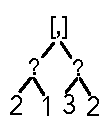
\includegraphics[scale=.25]{figures/tree1.pdf}
\smallskip

\noindent
At each choice point we can go either left or right; making such a decision
at each point leads to visiting one particular tuple.

\medskip
{\small
\begin{tabular}{@{}l@{~}ll@{~}ll@{~}ll@{~}l}
\begin{minipage}{1.2cm}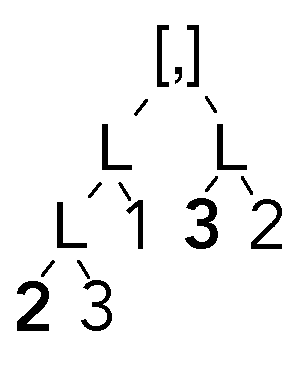
\includegraphics[scale=.25]{figures/tree2.pdf} 
\end{minipage} &  $ =   \tuple{p_2,p_3} $ &
\begin{minipage}{1.2cm}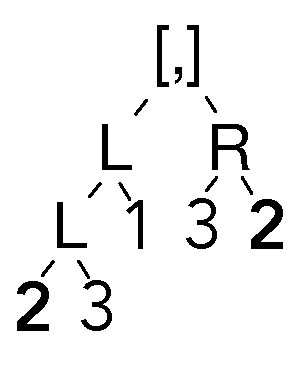
\includegraphics[scale=.25]{figures/tree3.pdf} 
\end{minipage} &  $ =   \tuple{p_2,p_2} $ 
&\begin{minipage}{1.2cm}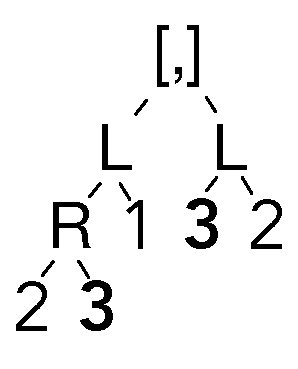
\includegraphics[scale=.25]{figures/tree4.pdf} 
\end{minipage} &  $ =   \tuple{p_3,p_3} $ \\
\begin{minipage}{1.2cm}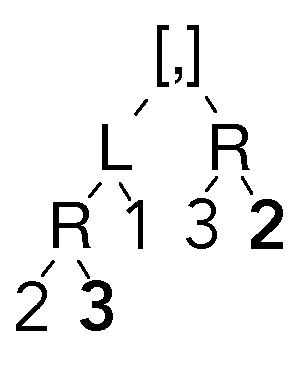
\includegraphics[scale=.25]{figures/tree5.pdf} 
\end{minipage} &  $ =   \tuple{p_3,p_2} $  &
\begin{minipage}{1.2cm}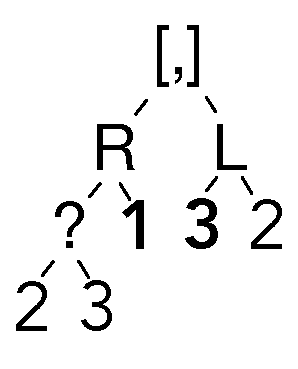
\includegraphics[scale=.25]{figures/tree6.pdf} 
\end{minipage} &  $ =   \tuple{p_1,p_3} $ 
&\begin{minipage}{1.2cm}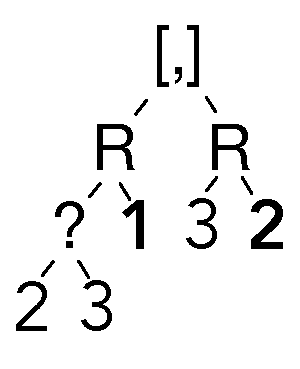
\includegraphics[scale=.25]{figures/tree7.pdf} 
\end{minipage} &  $ =   \tuple{p_1,p_2} $ 
\end{tabular}}

\medskip
\noindent 
Each tuple is uniquely determined by the original type term $t$ and a choice
string $c$. In the above example, the result of iteration through the
normalized, union-free, type terms is defined by the strings \L\L\L, \L\L\R,
\L\R\L, \L\R\R, \R\L, \R\R. The length of each string is bounded by the
number of unions in a term.


The iteration sequence in the above example is thus \L\L\uL $\rightarrow$
\L\uL\R $\rightarrow$ \L\R\uL $\rightarrow$ \uL\R\R $\rightarrow$ \R\uL
$\rightarrow$ \R\R, where the underlined choice is next one to be toggled in
that step. Stepping from a choice string $c$ to the next string consists of
splitting $c$ in three, $c' \,\L\,c''$, where $c'$ can be empty and $c''$ is a
possibly empty sequence of {\R}s.  The next string is $c'\, \R \, c_{pad}$,
that is to say it retains the prefix $c'$, toggles the \L to an \R, and is
padded by a sequence of \Ls. The leftover tail $c''$ is discarded. If there is
no \L in $c$, iteration terminates.

One step of iteration is performed by calling the \c{next} function with a
type term and a choice string (encoded as a \c{list} of \c{choice}\hspace{-0.25em}s); \c{next} either returns the next string in
the sequence or \c{None}. Internally, it calls \c{step} to toggle the
last \L and shorten the string (constructing $c'\,\R$). Then it calls on
\c{pad} to add the trailing sequence of \Ls (constructing $c'\,\R\,c_{pad}$).

\begin{lstlisting}
type choice = L | R

let rec next(a:typ)(l:choice list) = 
  match step l with
   | None -> None
   | Some(l') -> Some(fst (pad a l'))
\end{lstlisting}
\newpage

\noindent
The \c{step} function delegates the job of flipping the last occurrence of
\L to \c{toggle}. For ease of programming, it reverses the string so that
\c{toggle} can be a simple recursion without an accumulator.  If the given
string has no \L, then \c{toggle} returns empty and \c{step} returns
\c{None}.

\begin{lstlisting}
let step(l:choice list) =
  match rev (toggle (rev l)) with
  | [] -> None
  | hd::tl -> Some(hd::tl)

let rec toggle = function
  | [] -> []    
  | L::tl -> R::tl
  | R::tl -> toggle tl
\end{lstlisting}

\noindent The \c{pad} function takes a type term and a choice string to be
padded. It returns a pair, whose first element is the padded string and second
element is the string left over from the current type. Each union encountered
by \c{pad} in its traversal of the type consumes a character from the input
string. Unions explored after the exhaustion of the original choice string are
treated as if there was an \L remaining in the choice string. The first
component of the returned value is the original choice string
extended with an \L for every union encountered after exhaustion of the original.

\begin{lstlisting}
let rec pad t l =
   match t,l with
   | (Prim i,l) -> ([],l)
   | (Tuple(t,t'),l) -> 
      let (h,tl) = pad t l in
      let (h',tl') = pad t' tl in (h @ h',tl')
   | (Union(t,_),L::r) -> 
      let (h,tl) = pad t r in (L::h,tl)
   | (Union(_,t),R::r) -> 
      let (h,tl) = pad t r in (R::h,tl)
   | (Union(t,_),[]) -> (L::(fst(pad t [])),[])
\end{lstlisting}

\noindent
To obtain the initial choice string, the string composed solely of \Ls, it
suffices to call \c{pad} with the type term under consideration and an empty
list. The first element of the returned tuple is the initial choice
string. For convenience, we define the function \c{initial} for this.

\begin{lstlisting}
let initial(t:typ) = fst (pad t [])
\end{lstlisting}

%%%%%%%%%%%%%%%%%%%%%%%%%%%%%%%%%%%%%%
\subsection{Subtyping with iteration}

Julia's subtyping algorithm visits union-free type terms using choice
strings to iterate over types. The \c{subtype} function takes two type
terms, \c a and \c b, and returns true if they are related by
subtyping. It does so by iterating over all union-free type terms $t_a$ in \c a,
and checking that for each of them, there exists a union-free type term $t_b$ in
\c b such that $t_a <: t_b$.

\begin{lstlisting}
let subtype(a:typ)(b:typ) = allexist a b (initial a)
\end{lstlisting}

\noindent
The \c{allexist} function takes two type terms, \c a and \c b, and a choice
string \c f, and returns true if \c a is a subtype of \c b for the iteration
sequence starting at \c f. This is achieved by recursively testing that for
each union-free type term in \c a (induced by \c a and the current value of
\c f), there exists a union-free super-type in \c b.


\begin{lstlisting}
let rec allexist(a:typ)(b:typ)(f:choice list) =
  match exist a b f (initial b) with 
  | true -> (match next a f with
             | Some ns -> allexist a b ns 
             | None -> true) 
  | false -> false
\end{lstlisting}

\noindent
Similarly, the \c{exist} function takes two type terms, \c a and \c b, and
choice strings, \c f and \c e. It returns true if there exists in \c b, a
union-free super-type of the type specified by \c f in \c a. This is done by
recursively iterating through \c e. The determination if two terms are
related is delegated to the \c{sub} function.

\begin{lstlisting}
type res = NotSub | IsSub of choice list * choice list

let rec exist(a:typ)(b:typ)(f:choice list)(e:choice list) =
  match sub a b f e with 
  | IsSub(_,_) -> true 
  | NotSub -> 
     (match next b e with
      | Some ns -> exist a b f ns 
      | None -> false) 
\end{lstlisting}

\noindent
Finally, the \c{sub} function takes two type terms and choice strings and
returns a value of type \c{res}. A \c{res} can be either \c{NotSub}, indicating that the
types are not subtypes, or \c{IsSub(_,_)} when they are subtypes. If the two types
are primitives, then they are only subtypes if they are equal. If the types
are tuples, they are subtypes if each of their respective elements are subtypes. Note
that the return type of \c{sub}, when successful, holds the unused choice
strings for both type arguments. When encountering a union, \c{sub} 
follows the choice strings to decide which branch to take. Consider, for
instance, the case when the first type term is \c{Union(t1,t2)} and the
second is type \c{t}. If the first element of the choice string is an \L,
then \c{t1} and \c{t} are checked, otherwise \c{sub} checks \c{t2}
and \c{t}.

\begin{lstlisting}
let rec sub t1 t2 f e =
  match t1,t2,f,e with 
  | (Prim i,Prim j,f,e) -> if i==j then IsSub(f,e) else NotSub
  | (Tuple(a1,a2), Tuple(b1,b2),f,e) ->
     (match sub a1 b1 f e with
      | IsSub(f', e') -> sub a2 b2 f' e'
      | NotSub -> NotSub)
  | (Union(a,_),b,L::f,e) -> sub a b f e
  | (Union(_,a),b,R::f,e) -> sub a b f e
  | (a,Union(b,_),f,L::e) -> sub a b f e
  | (a,Union(_,b),f,R::e) -> sub a b f e
\end{lstlisting}

%%%%%%%%%%%%%%%%%%%%%%%%%%%%%%%%%%%%%%
\subsection{Further optimization}

This implementation represents choice strings as linked lists, but this design
requires allocation and reversals when stepping. However, the implementation
can be made more efficient by using a mutable bit vector instead of a linked
list. Additionally, the maximum length of the bit vector is bounded by the
number of unions in the type, so it need only be allocated once. Julia's
implementation uses this efficient representation.

%%%%%%%%%%%%%%%%%%%%%%%%%%%%%%%%%%%%%%
%%%%%%%%%%%%%%%%%%%%%%%%%%%%%%%%%%%%%%
%%%%%%%%%%%%%%%%%%%%%%%%%%%%%%%%%%%%%%
\section{Correctness and completeness of subtyping}

To prove the correctness of Julia's subtyping, we take the following general
approach. We start by giving a denotational semantics for types from which
we derive a definition of semantic subtyping. Then we easily prove that a
normalization-based subtyping algorithm is correct and complete. This provides
the general framework for which we prove two iterator-based algorithms correct.
The first iterator-based algorithm explicitly includes the structure of the type in
its state to guide iteration; the second is identical to that of the prior section.

The order in which choice strings iterate through a type term is determined by
both the choice string and the type term being iterated over. Rather than
directly working with choice strings as iterators over types,
we start with a simpler structure, namely that of iterators over the trees
induced by type terms. We prove correct and complete a subtyping algorithm
that uses these simpler iterators. Finally, we establish a correspondence 
between tree iterators and choice string iterators. This concludes our proof
of correctness and completeness, and details can be found in the Coq
mechanization.

The denotational semantics we use for types is as follows:

\vspace{-5mm}
\begin{align*}
\denotes{p_i} &= \{p_i\} \\
\denotes{\union{t_1}{t_2}} &= \denotes{t_1} \cup \denotes{t_2} \\
\denotes{\tuplet{t_1}{t_2}} &= \{\tuplet{t'_1}{t'_2} \,|\, t_1' \in \denotes{t_1},  t_2' \in \denotes{t_2'}\}
\end{align*}
\vspace{-5mm}

\noindent
We define subtyping as follows: if $\denotes{t}\subseteq\denotes{t'}$, then
$t<:t'$.  This leads to the definition of subtyping in our restricted language.

\begin{definition}
 The subtyping relation $t_1 <: t_2$ holds iff $\forall t_1' \in
\denotes{t_1}, \exists\, t_2' \in \denotes{t_2}, t_1' =
t_2'$.\label{dfn:scr}
\end{definition}

\noindent
The use of equality for relating types is a simplification afforded by the
structure of primitives.

%%%%%%%%%%%%%%%%%%%%%%%%%%%%%%%%%%%%%%%%%%
\subsection{Subtyping with normalization}

The correctness and completeness of the normalization-based subtyping
algorithm requires proving that the \c{norm}
function returns all union-free type terms.

\begin{lemma}[NF Equivalence]\label{lem:equiv_ndet}
$t' \in \denotes{t}$ iff $t' \in \c{norm}~ t$.
\end{lemma}

\noindent
Theorem~\ref{nsf} states that the \c{subtype} relation of
Section~\ref{norm} abides by Definition~\ref{dfn:scr} because it uses
\c{norm} to compute the set of union-free type terms for both argument
types, and directly checks subtyping.

\begin{theorem}[NF Subtyping]\label{nsf}
For all  a and b, \c{subtype} a b iff $a <: b$.
\end{theorem}

\noindent
Therefore, normalization-based subtyping is correct against our definition.


%%%%%%%%%%%%%%%%%%%%%%%%%%%%%%%%%%%%%%
\subsection{Subtyping with tree iterators}

Reasoning about iterators that use choice strings, as described in
Section~\ref{cs}, is tricky as it requires simultaneously reasoning about
the structure of the type term and the validity of the choice string that
represents the iterator's state. Instead, we propose to use an intermediate
data structure, called a tree iterator, to guarantee consistency of iterator
state with type structure.

A tree iterator is a representation of the iteration state embedded in a type
term. Thus a tree iterator yields a union-free tuple and can either step to a
successor state or a final state. Recalling the graphical notation of
Section~\ref{cs}, we can represent the state of iteration as a combination of
type term and a choice or, equivalently, as a tree iterator.

\medskip
{\small
\begin{tabular}{@{}l@{~}ll@{~}ll@{~}ll@{~}l}
\it Choice string: &&  \multicolumn{2}{l}{\it Tree iterator:}\\[2mm]
\begin{minipage}{1.2cm}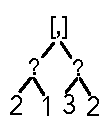
\includegraphics[scale=.25]{figures/tree1.pdf} 
\end{minipage} , \R\L & $ =   \tuple{p_1,p_3} $ 
&\begin{minipage}{1.2cm}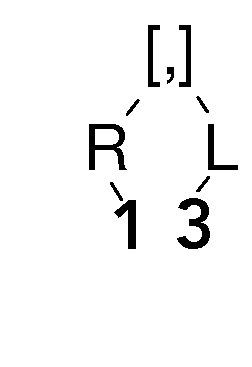
\includegraphics[scale=.25]{figures/tree8.pdf}
\end{minipage}& $=\tuple{p_1,p_3}$
\end{tabular}}

\noindent
This structure-dependent construction makes tree iterators less efficient
than choice strings. A tree iterator must have a node for each structural
element of the type being iterated over, and is thus less space efficient
than the simple choices-only strings. However, it is easier to prove
subtyping correct for tree iterators first.

Tree iterators depend on the type term they iterate over. The possible
states are \c{IPrim} at primitives, \c{ITuple} at tuples, and for unions
either \c{ILeft} or \c{IRight}.

\begin{lstlisting}
Inductive iter: Typ -> Set :=
| IPrim : forall i, iter (Prim i)
| ITuple : forall t1 t2, iter t1 -> iter t2 -> iter (Tuple t1 t2)
| ILeft : forall t1 t2, iter t1 -> iter (Union t1 t2)
| IRight : forall t1 t2, iter t2 -> iter (Union t1 t2).
\end{lstlisting}

\noindent
The \c{next} function for tree iterators steps in depth-first,
right-to-left order. There are four cases to consider:
\begin{itemize}
  \item A primitive has no successor.
  \item A tuple steps its second child; if that
has no successor step, then it steps its first child and resets the second
child.
  \item An \c{ILeft} tries to step its child. If it has no successor, then the \c{ILeft} becomes an \c{IRight} with a newly initialized child corresponding to the right child of the union.
  \item An \c{IRight} also tries to step its child, but is final if its child has no successor.
  \end{itemize}

\begin{lstlisting}
Fixpoint next(t:Typ)(i:iter t): option(iter t) := match i with
  | IPrim _ => None
  | ITuple t1 t2 i1 i2 =>
    match (next t2 i2) with
    | Some i' => Some(ITuple t1 t2 i1 i')
    | None =>
      match (next t1 i1) with
      | Some i' => Some(ITuple t1 t2 i' (start t2))
      | None => None
      end
    end
  | ILeft t1 t2 i1 =>
    match (next t1 i1) with
    | Some(i') => Some(ILeft t1 t2 i')
    | None => Some(IRight t1 t2 (start t2))
    end
  | IRight t1 t2 i2 => 
    match (next t2 i2) with
    | Some(i') => Some(IRight t1 t2 i')
    | None => None
    end
  end.
\end{lstlisting}
% todo: describe induction principle 
% text just below theorem 4 is sensible but could be expanded a bit
% put theorems below figure 

\noindent
An induction principle for tree iterators is needed to reason about all
iterator states for a given type. First, we show that iterators eventually
reach a final state. This is done with a function \c{inum}, which assigns
natural numbers to each state. It simply counts the number of remaining
steps in the iterator. To count the total number of union-free types 
denoted by a type, we use the \c{tnum} helper function.

\begin{lstlisting}
Fixpoint tnum(t:Typ):nat :=
  match t with
  | Prim i => 1
  | Tuple t1 t2 => tnum t1 * tnum t2
  | Union t1 t2 => tnum t1 + tnum t2
  end.

Fixpoint inum(t:Typ)(ti:iter t):nat :=
  match ti with
  | IPrim i => 0
  | ITuple t1 t2 i1 i2 => inum t1 i1 * tnum t2 + inum t2 i2
  | IUnionL t1 t2 i1 => inum t1 i1 + tnum t2
  | IUnionR t1 t2 i2 => inum t2 i2
  end.
\end{lstlisting}

\noindent This function then lets us define the key theorem needed for the
induction principle. At each step, the value of \c{inum} decreases by 1, and
since it cannot be negative, the iterator must therefore reach a final
state.

\begin{lemma}[Monotonicity]\label{inum_mono}
If $\c{next}~t~it = it'$ then $\c{inum}~t~it = 1 + \c{inum}~t~it'$.
\end{lemma}

\noindent
It is now possible to define an induction principle over \c{next}. By
monotonicity, \c{next} eventually reaches a final state.  For any property
of interest, if we prove that it holds for the final state and for the
induction step, we can prove it holds for every state for that type.

\begin{theorem}[Tree Iterator Induction]\label{indprop}
Let $P$ be any property of tree iterators for some type $t$.  Suppose $P$
holds for the final state, and whenever $P$ holds for a successor state $it$
then it holds for its precursor $it'$ where $\c{next}~t~it' = it$.  Then $P$
holds for every iterator state over $t$.
\end{theorem} 

\noindent Now, we can prove correctness of the subtyping algorithm with tree
iterators. We implement subtyping with respect to choice strings in the Coq
implementation in a two-stage process. First, we compute the union-free types
induced by the iterators over their original types using \c{here}. Second, we
decide subtyping between the two union-free types in \c{ufsub}. The function
\c{here} walks the given iterator, producing a union-free type mirroring its
state.  To decide subtyping between the resulting union-free types, \c{ufsub}
checks equality between \c{Prim}\hspace{-0.3em}s and recurses on the elements
of \c{Tuple}\hspace{-0.3em}s, while returning false for all other types. Since
\c{here} will never produce a union type, the case of \c{ufsub} for them is
irrelevant, and is false by default.

\medskip

\noindent
\begin{minipage}{0.53\textwidth}
\begin{lstlisting}
Fixpoint here(t:Typ)(i:iter t):Typ:=
  match i with
  | IPrim i => Prim i
  | ITuple t1 t2 p1 p2 => 
    Tuple (here t1 p1) (here t2 p2)
  | ILeft t1 t2 pl => (here t1 pl)
  | IRight t1 t2 pr => (here t2 pr)
  end.
\end{lstlisting}
\end{minipage}
\begin{minipage}{0.47\textwidth}
\begin{lstlisting}[escapechar=\%]
Fixpoint ufsub(t1 t2:Typ) :=
  match (t1, t2) with
  | (Prim p, Prim p') => p==p'
  | (Tuple a a', Tuple b b') =>
      ufsub a b && ufsub a' b'
  | (_, _) => false
  end.
%
\end{lstlisting}
\end{minipage}


\begin{lstlisting}
Definition sub (a b:Typ) (ai:iter a) (bi:iter b) :=
    ufsub (here a ai) (here b bi).
\end{lstlisting}

\noindent This version of \c{sub} differs from the algorithmic implementation to
ensure that recursion is well founded. The previous version of \c{sub} was, in
the case of unions, decreasing on alternating arguments  when unions were
found on either of the sides. In contrast, the proof's version of \c{sub}
applies the choice string to each side first using \c{here}, a strictly
decreasing function that recurs structurally on the given type. This computes
the union-free type induced by the iterator applied to the current
type. The algorithm then checks subtyping between the resultant union-free
types, which is entirely structural. These implementations are equivalent, as
they both apply the given choice strings at the same places while computing
subtyping; however, the proof version separates choice string application
while the implementation intertwines it with the actual subtyping decision.

Versions of \c{exist} and \c{allexist} that use tree iterators are given
next. They are similar to the string iterator functions of Section~\ref{cs}.
\c{exist} tests if the subtyping relation holds in the context of the
current iterator states for both sides. If not, it recurs on the next
state. Similarly, \c{allexist} uses its iterator for $a$ in conjunction with
\c{exist} to ensure that the current left-hand iterator state has a matching
right-hand state. We prove termination of both using Lemma~\ref{inum_mono}.

\begin{lstlisting}
Definition subtype(a b:Typ) = allexist a b (initial a)

Program Fixpoint allexist (a b:typ)(ia:iter a) {measure(inum ia)} =
   exists a b ia (initial b) && 
      (match next a ia with 
       | Some(ia') => allexist a b ia' 
       | None => true).

Program Fixpoint exist(a b:typ)(ia:iter a)(ib:iter b)
                                      {measure(inum ib)} =
   subtype a b ia ib  || 
      (match next b ib with 
       | Some(ib') => exist a b ia ib' 
       | None => false).
\end{lstlisting}

\newcommand{\irdn}[1]{\ensuremath{\mathcal{R}({#1})}}
\newcommand{\irch}[2]{\ensuremath{|#1|_{#2}}}

\noindent
The denotation of a tree iterator state $\irdn{i}$ is the set of states that
can be reached using \c{next} from $i$. Let $a(i)$ indicate the union-free
type produced from the type $a$ at $i$, and \irch{i}{a} is the set
$\{a(i')\,|\,i'\in\irdn{i}\}$, the union-free types that result from states
in the type $a$ reachable by $i$.  This lets us prove that the set of types
corresponding to states reachable from the initial state of an iterator is
equal to the set of states denoted by the type itself.

\begin{lemma}[Initial equivalence]\label{triter_eq}
$\irch{\c{initial}~a}{a} = \denotes{a}$.
\end{lemma}

\noindent
Next, Theorem~\ref{indprop} allows us to show that \c{exists} of $a$, $b$,
with $i_a$ and $i_b$  tries to find an iterator state $i_b'$ starting from
$i_b$ such that $b(i_b') = a(i_a)$. The desired property trivially holds
when $\irch{i_b}{b} = \emptyset$, and if the iterator can step then either
the current union-free type is satisfying or we defer to the induction
hypothesis.


\begin{theorem}\label{trexcor}
$\c{exist}\;a\;b\;i_a\;i_b$ holds iff $\exists t\in\irch{i_b}{b},a(i_a)= t$.
\end{theorem}

\noindent
We can then appeal to both Theorem~\ref{trexcor} and Lemma~\ref{triter_eq}
to show that $\c{exist}\;a\;b\;i_a\;(\c{initial}\;b)$ finds a satisfying
union-free type on the right-hand side if it exists in $\denotes{b}$. Using
this, we can then use Theorem~\ref{indprop} in an analogous way to \c{exist}
to show that \c{allexist} is correct up to the current iterator state.

\begin{theorem}\label{trfacor}
$\c{allexist}\;a\;b\;i_a$ holds iff $\forall a'\in \irch{i_a}{a},
  \exists b'\in \denotes{b}, a'= b'$.
\end{theorem}

\noindent
Finally, we can appeal to Theorem~\ref{trfacor} and Lemma~\ref{triter_eq}
again to show correctness of  the algorithm.

\begin{theorem}
$\c{subtype}\;a\;b$ holds iff $\forall a' \in \denotes{a}, \exists b' \in
  \denotes{b}, a' = b'$.
\end{theorem}

%%%%%%%%%%%%%%%%%%%%%%%%%%%%%%%%%%%%%%
\subsection{Subtyping with choice strings}

We prove the subtyping algorithm using choice strings correct and complete. We
start by showing that iterators over choice strings simulate tree iterators. 
This lets us prove that the choice string based subtyping algorithm is correct
by showing that the iterators at each step are equivalent.
To relate tree iterators to choice string iterators, we use the \c{itp}
function, which traverses a tree iterator state and linearizes it, producing a
choice string using depth-first search.


\begin{lstlisting}
Fixpoint itp{t:Typ}(it:iter t):choice list :=
   match it with
   | IPrim _ => nil
   | ITuple t1 t2 it1 it2 => (itp t1 it1)++(itp t2 it2)
   | ILeft t1 _ it1 => Left::(itp t1 it1)
   | IRight _ t2 it1 => Right::(itp t2 it1)
   end.
\end{lstlisting}

\noindent Next, we define an induction principle over choice strings by way of
linearized tree iterators. The \c{next} function in Section~\ref{cs} works by
finding the last \L in the choice string, turning it into an \R, and replacing
the rest with \Ls until the type is valid. If we use \c{itp} to translate
both the initial and final states for a valid \c{next} step of a tree
iterator, we see the same structure.

\begin{lemma}[Linearized Iteration]
\label{lem:snt}
For some type $t$ and tree iterators $\mathit{it}\,\mathit{it}'$, if
$\c{next}\,t\,\mathit{it}=\mathit{it'}$, there exists some prefix  $c'$, an
initial suffix $c''$ made up of \Rs, and a final suffix  $c'''$
consisting of \Ls such that $\c{itp}~t~it=c'\,\c{Left}\,c''$ and 
$\c{itp}~t~it'=c'\,\c{Right}\,c'''$.
\end{lemma}

\noindent
We can then prove that stepping a tree iterator state is equivalent to
stepping the linearized versions of the state using the choice string
\c{next} function.

\begin{lemma}[Step Equivalence]\label{sctxcorr}
If $\mathit{it}$ and $\mathit{it'}$ are tree iterator states and
$\c{next}~\mathit{it}=\mathit{it}'$, then $\c{next} (\c{itp}\;\mathit{it}) =
(\c{itp}\;\mathit{it'})$.
\end{lemma}
\noindent
The initial state of a tree iterator linearizes to the
initial state of a choice string iterator.

\begin{lemma}[Initial Equivalence]\label{eqinit}
$\c{itp} (\c{initial}\;t) = \c{pad}\;t\;\c{[]}$.
\end{lemma}

\noindent
The functions \verb|exist| and \verb|allexist| for choice string based
iterators are identical to those for tree iterators (though using choice
string iterators internally), and \verb|sub| is as described in
Section~\ref{cs}. The correctness proofs for the choice string subtype
decision functions use the tree iterator induction principle
(Theorem~\ref{indprop}), and are thus in terms of tree iterators. By
Lemma~\ref{sctxcorr}, however, each step that the tree iterator takes will be
mirrored precisely by \c{itp} into choice strings. Similarly, the initial states
are identical by Lemma~\ref{eqinit}. As a result, the sequence of states
checked by each of the iterators is equivalent with \c{itp}.

\begin{lemma}\label{cstrec}
$\c{exist}~a~b~(\c{itp}~i_a)~(\c{itp}~i_b)$ holds iff $\exists t \in
  \irch{i_b}{b}, a(ia)=t$.
\end{lemma}

\noindent With the correctness of \c{exist} following from the tree iterator
definition, we can apply the same proof methodology to show that \c{allexist}
is correct. In order to do so, we instantiate Lemma~\ref{cstrec}  with
Lemma~\ref{triter_eq} and Lemma~\ref{eqinit} to show that if $\c{exist}\;\c
a\;\c b\;(\c{itp}\;\c{ia})\;(\c{pad}\;\c t\;\c{[]})$ then $\exists \c t \in
\denotes{\c b}, \c a(\c{ia}) = \c t$, allowing us to check  each of the exists
cases while establishing the forall-exists relationship.

\begin{lemma}\label{cstraec}
$\c{allexist}~a~b~(\c{itp}~i_a)$
 holds iff $\forall a'\in\irch{i_a}{a}, \exists b'\in\denotes{b},a'=b'$.
\end{lemma}

\noindent We can then instantiate Lemma~\ref{cstraec} with
Lemma~\ref{eqinit} and Lemma~\ref{triter_eq} to show that \c{allexist} for
choice strings ensures that the forall-exists relation holds.
 
\begin{theorem}
$\c{allexist}~a~b~(\c{pad}~t~\c{[]})$
 holds iff $\forall a'\in\denotes{a},\exists b'\in\denotes{b}, a'=b'$.
\end{theorem}

\noindent Finally, we can prove that subtyping is correct using the choice
string algorithm.

\begin{theorem}
$\c{subtype}~a~b$ holds iff $\forall a'\in\denotes{a}, \exists
  b'\in\denotes{b}, a'=b'$.
\end{theorem}

\noindent
Thus, we can correctly decide subtyping with distributive unions and tuples
using the choice string based implementation of iterators.

\section{Complexity}

The worst-case time complexity of Julia's subtyping algorithm and
normalization-based approaches is determined by the number of terms that
could exist in the normalized type. In the worst case, there are $2^n$
union-free tuples in the fully normalized version of a type that has $n$
unions.  Each of those tuples must always be explored. As a result, both
algorithms have worst-case $O(2^n)$ time complexity. The approaches differ,
however, in space complexity. The normalization approach computes and stores
each of the exponentially many alternatives, so it also has $O(2^n)$ space
complexity. However, Julia need only store the choice made at each union,
thereby offering $O(n)$ space complexity.

Julia's algorithm improves best-case time performance.  Normalization always
experiences worst-case time and space behavior as it has to precompute the
entire normalized type. Julia's iteration-based algorithm can discover the
relation between types early. In practice, many queries are of the form
$\mathit{uft} <: union(t_1...t_n)$, where $\mathit{uft}$ is an already
union-free tuple. As a result, all that Julia needs to do is find one matching
tuple in $t_1 ... t_n$, which can be done sequentially without needing explicit
enumeration.

\section{Future work}

We plan to handle additional features of Julia. Our
next steps will be subtyping for primitive types, existential type variables,
and invariant constructors.  Adding subtyping to primitive types would be the
simplest change. The challenge is how to retain completeness, as a primitive
subtype heirarchy and semantic subtyping have undesirable interactions.  For
example, if the primitive subtype hierarchy contains only the relations $p_2
\sub p_1$ and $p_3 \sub p_1$, then is $p_1$ a subtype of $\union{p_2}{p_3}$?
In a semantic subtyping system, they are, but this requires changes both to
the denotational framework and the search space of the iterators.  Existential
type variables create substantial new complexities in the state of the
algorithm. No longer is the state solely restricted to that of the iterators
being attempted; now, the state includes variable bounds that are accumulated
as the algorithm compares types to type variables. As a result, correctness
becomes a much more complex contextually linked property to prove.  Finally,
invariant type constructors induce contravariant subtyping, which when
combined with existential variables may create cycles within the subtyping
relation.  

\section{Conclusion} It is likely that subtyping with unions and tuples is
always going to be exponential time, as subtyping of regular expression types
have been proven to be EXPTIME-complete~\cite{unionexptime}. However, it need
not take exponential space to decide subtyping: we have described and proven
correct a subtyping algorithm for covariant tuples and unions that uses
iterators instead of normalization. This algorithm uses linear space and
allows common patterns, such as testing if a tuple of primitives is a subtype
of a tuple of unions, to be handled as a special case of the subtyping
algorithm. Finally, based on Julia's experience with the algorithm, we think
that it can generalize to rich type languages; Julia supports bounded
polymorphism and invariant constructors enabled in part by its use of this
algorithm.



\medskip

\subsubsection*{Acknowledgments} The authors thank Jiahao Chen for starting us
down the path of understanding Julia, and Jeff Bezanson for coming up with
Julia's subtyping algorithm. We would  also like to thank Ming-Ho Yee, Celeste
Hollenbeck, and Julia Belyakova for their help in preparing this paper. This
work received funding from the European Research Council under the European
Union's Horizon 2020 research and innovation programme (grant agreement
695412), the NSF (award 1544542 and award 1518844), the ONR (grant 503353),
and the Czech Ministry of Education, Youth and Sports (grant agreement
CZ.02.1.01/0.0/0.0/15\_003/0000421).
 

%\bibliographystyle{plain}
\bibliography{refs}
\end{document}
